\documentclass{article}

% content/resources/templates/preamble.tex
\usepackage[margin=0.6in]{geometry}
\author{Milav Dabgar}
\usepackage{amsmath,amssymb,amsthm}
\usepackage{booktabs}
\usepackage{multirow}
\usepackage{xcolor}
\usepackage{tcolorbox}
\tcbuselibrary{breakable,skins}
\usepackage[colorlinks=true,linkcolor=blue]{hyperref}
\usepackage{titlesec}
\usepackage{enumitem}
\usepackage{tikz}
\usepackage{pgfplots}
\usepackage{circuitikz}
\usepackage[version=4]{mhchem}
\usepackage{longtable}
\usepackage{array}
\usepackage{float}
\usepackage{caption}
\usepackage{listings}

\lstset{
  basicstyle=\small\ttfamily,
  breaklines=true,
  breakatwhitespace=false,
  postbreak=\mbox{\textcolor{red}{$\hookrightarrow$}\space},
  float=false,
  numbers=left,
  numberstyle=\tiny\color{gray},
  numbersep=10pt,
  xleftmargin=2em,
  keywordstyle=\color{blue},
  commentstyle=\color{green!60!black},
  stringstyle=\color{purple},
  backgroundcolor=\color{gray!5},
  showstringspaces=false,
  tabsize=2,
  captionpos=b,
  keepspaces=true,
  columns=flexible
}

\pgfplotsset{compat=1.18}
\usetikzlibrary{shapes,arrows,positioning,calc,patterns,decorations.pathmorphing,decorations.markings,arrows.meta}

% Color scheme
\definecolor{headcolor}{RGB}{0,102,204}
\definecolor{keycolor}{RGB}{220,20,60}
\definecolor{solutioncolor}{RGB}{34,139,34}
\definecolor{mnemoniccolor}{RGB}{148,0,211}
\definecolor{codecolor}{RGB}{0,0,100}

% Spacing
\setlength{\parskip}{3pt}
\setlist[itemize]{nosep}
\setlist[enumerate]{nosep}

% Title formatting
\titleformat{\section}{\Large\bfseries\color{headcolor}}{\thesection}{1em}{}
\titleformat{\subsection}{\large\bfseries\color{headcolor}}{\thesubsection}{1em}{}

% Pandoc tightlist compatibility
\providecommand{\tightlist}{%
  \setlength{\itemsep}{0pt}\setlength{\parskip}{0pt}}

% Pandoc longtable compatibility
\newcounter{none}
\def\thenone{}


% content/resources/templates/english-boxes.tex
% This file is currently empty - it exists to maintain consistency with the import structure.
% Add custom environments here if needed in the future.


% Custom commands for GTU solutions
% This file defines semantic commands for consistent formatting

% Question command with automatic formatting
\newcommand{\question}[2]{%
  \section*{Question #1}%
  \textbf{#2}%
}

% OR question variant
\newcommand{\questionor}[2]{%
  \section*{Question #1 OR}%
  \textbf{#2}%
}

% Proper table environment with caption
\newenvironment{answertable}[1]{%
  \begin{table}[htbp]
  \centering
  \caption{#1}
}{%
  \end{table}
}

% Proper figure environment for diagrams
\newenvironment{answerdiagram}[1]{%
  \begin{figure}[htbp]
  \centering
  \caption{#1}
}{%
  \end{figure}
}

% Semantic markup for key terms
\newcommand{\keyword}[1]{\textbf{#1}}
\newcommand{\code}[1]{\texttt{#1}}
\newcommand{\classname}[1]{\texttt{#1}}
\newcommand{\methodname}[1]{\texttt{#1}}

% Proper quotation marks
\newcommand{\mnemonic}[1]{``#1''}


\title{Fundamentals of Electrical Engineering (4311101) - Winter 2024 Solution}
\date{January 10, 2024}

\begin{document}
\maketitle

% Question 1
\questionmarks{1(a)}{3}{Define current, electric Power and energy.}

\begin{solutionbox}
\textbf{Answer}:

\begin{center}
\captionof{table}{Basic Electrical Terms}
\begin{tabulary}{\linewidth}{|L|L|}
\hline
\textbf{Term} & \textbf{Definition} \\ \hline
\textbf{Current} & The rate of flow of electric charge through a conductor (measured in amperes, A). \\ \hline
\textbf{Electric Power} & The rate at which electrical energy is transferred or consumed (measured in watts, W). \\ \hline
\textbf{Energy} & The capacity to do work, measured as power multiplied by time (measured in joules or watt-hours). \\ \hline
\end{tabulary}
\end{center}
\end{solutionbox}

\begin{mnemonicbox}
\mnemonic{CPE: Charge-Per-second, Product-of-VI, Energy-over-time}
\end{mnemonicbox}

\questionmarks{1(b)}{4}{Explain the effect of temperature on the value of resistance of pure metal, alloys and insulators.}

\begin{solutionbox}
\textbf{Answer}:

\begin{center}
\captionof{table}{Temperature Effect on Resistance}
\begin{tabulary}{\linewidth}{|L|L|L|}
\hline
\textbf{Material Type} & \textbf{Temperature Effect} & \textbf{Equation} \\ \hline
\textbf{Pure Metals} & Resistance increases with temperature (Positive Temperature Coefficient). & $R_2 = R_1[1 + \alpha(T_2-T_1)]$ \\ \hline
\textbf{Alloys} & Slight increase with temperature (Very low $\alpha$). & $R_2 = R_1[1 + \alpha(T_2-T_1)]$ \\ \hline
\textbf{Insulators} & Resistance decreases with temperature (Negative Temperature Coefficient). & $R_2 = R_1 e^{\beta(1/T_2-1/T_1)}$ \\ \hline
\end{tabulary}
\end{center}

Where $\alpha$ is the temperature coefficient, $T$ is temperature, and $R$ is resistance.
\end{solutionbox}

\begin{mnemonicbox}
\mnemonic{MAI: Metals Add, Alloys Increase-little, Insulators Invert}
\end{mnemonicbox}

\questionmarks{1(c)}{7}{State and explain KCL and KVL with examples.}

\begin{solutionbox}
\textbf{Answer}:

\textbf{Kirchhoff's Laws:}

\begin{center}
\captionof{table}{KCL vs KVL}
\begin{tabulary}{\linewidth}{|L|L|L|}
\hline
\textbf{Law} & \textbf{Statement} & \textbf{Equation} \\ \hline
\textbf{KCL} & Sum of currents entering a node equals sum of currents leaving the node. & $\sum I_{in} = \sum I_{out}$ \\ \hline
\textbf{KVL} & Sum of voltage drops equals sum of voltage rises in a closed loop. & $\sum V = 0$ \\ \hline
\end{tabulary}
\end{center}

\begin{answerdiagram}{KCL and KVL Illustrations}
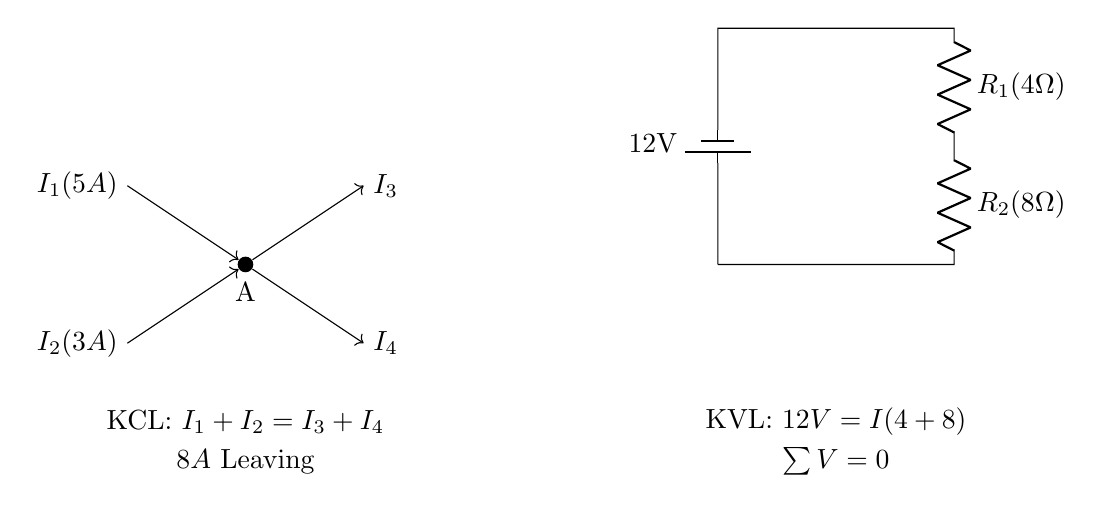
\begin{tikzpicture}
    % KCL
    \begin{scope}[xshift=0cm, yshift=0cm]
        \node[circle, fill=black, inner sep=2pt, label=below:A] (A) at (0,0) {};
        \draw[<-] (A) -- (-1.5, 1) node[left] {$I_1 (5A)$};
        \draw[<-] (A) -- (-1.5, -1) node[left] {$I_2 (3A)$};
        \draw[->] (A) -- (1.5, 1) node[right] {$I_3$};
        \draw[->] (A) -- (1.5, -1) node[right] {$I_4$};
        \node at (0, -2) {KCL: $I_1+I_2 = I_3+I_4$};
        \node at (0, -2.5) {$8A$ Leaving};
    \end{scope}

    % KVL
    \begin{scope}[xshift=6cm, yshift=0cm]
        \draw (0,0) to[battery1, l=12V] (0,3) -- (3,3) to[R, l=$R_1(4\Omega)$] (3,1.5) to[R, l=$R_2(8\Omega)$] (3,0) -- (0,0);
        \node at (1.5, -2) {KVL: $12V = I(4+8)$};
        \node at (1.5, -2.5) {$\sum V = 0$};
    \end{scope}
\end{tikzpicture}
\end{answerdiagram}

\textbf{Example}:
\begin{itemize}
    \item \keyword{KCL}: At node A, if $I_1 = 5A$ and $I_2 = 3A$ entering, then $I_3 + I_4 = 8A$ must be leaving.
    \item \keyword{KVL}: In a loop with battery 12V and resistors $R_1(4\Omega)$ and $R_2(8\Omega)$, $12V = I(4\Omega+8\Omega)$.
\end{itemize}
\end{solutionbox}

\begin{mnemonicbox}
\mnemonic{CLAN: Currents Leave And eNter equally, Voltage Around Loop is Null}
\end{mnemonicbox}

% Question 1 OR
\questionmarks{1(c) OR}{7}{Explain series and parallel connections of resistors with necessary equations.}

\begin{solutionbox}
\textbf{Answer}:

\begin{center}
\captionof{table}{Series vs Parallel Connections}
\begin{tabulary}{\linewidth}{|L|L|L|}
\hline
\textbf{Connection} & \textbf{Equation} & \textbf{Characteristics} \\ \hline
\textbf{Series} & $R_{eq} = R_1 + R_2 + R_3 + \dots + R_n$ & Same current through all resistors. Total R increases. \\ \hline
\textbf{Parallel} & $\frac{1}{R_{eq}} = \frac{1}{R_1} + \frac{1}{R_2} + \frac{1}{R_3} + \dots + \frac{1}{R_n}$ & Same voltage across all resistors. Total R decreases. \\ \hline
\end{tabulary}
\end{center}

\begin{answerdiagram}{Resistor Connections}
\begin{circuitikz}[scale=0.8, transform shape]
    % Series
    \draw (0,2) to[R, l=$R_1$] (2,2) to[R, l=$R_2$] (4,2) to[R, l=$R_3$] (6,2);
    \node at (3, 1) {Series: Current $I$ constant};

    % Parallel
    \begin{scope}[yshift=-2cm]
        \draw (0,0) -- (1,0) -- (1,1.5) to[R, l=$R_1$] (5,1.5) -- (5,0) -- (6,0);
        \draw (1,0) -- (1,0) to[R, l=$R_2$] (5,0) -- (5,0);
        \draw (1,0) -- (1,-1.5) to[R, l=$R_3$] (5,-1.5) -- (5,0);
        \node at (3, -2.5) {Parallel: Voltage $V$ constant};
    \end{scope}
\end{circuitikz}
\end{answerdiagram}
\end{solutionbox}

\begin{mnemonicbox}
\mnemonic{SPARC: Series Plus All Resistors, parallel Combines with reciprocals}
\end{mnemonicbox}

% Question 2
\questionmarks{2(a)}{3}{Write factors affecting the Resistance value.}

\begin{solutionbox}
\textbf{Answer}:

The resistance $R$ of a conductor depends on:

\begin{center}
\captionof{table}{Factors Affecting Resistance}
\begin{tabulary}{\linewidth}{|L|L|L|}
\hline
\textbf{Factor} & \textbf{Effect on Resistance} & \textbf{Relation} \\ \hline
\textbf{Length ($l$)} & Directly proportional & $R \propto l$ \\ \hline
\textbf{Cross-sectional Area ($A$)} & Inversely proportional & $R \propto 1/A$ \\ \hline
\textbf{Material ($\rho$)} & Depends on resistivity & $R \propto \rho$ \\ \hline
\textbf{Temperature ($T$)} & Usually increases with temperature & $R \propto T$ \\ \hline
\end{tabulary}
\end{center}

\keyword{Combined Formula}: $R = \rho \frac{l}{A}$
\end{solutionbox}

\begin{mnemonicbox}
\mnemonic{LAMT: Length Adds, Area Minimizes, Material matters, Temperature transforms}
\end{mnemonicbox}

\questionmarks{2(b)}{4}{Draw power triangle and define active and reactive power.}

\begin{solutionbox}
\textbf{Answer}:

\begin{center}
\captionof{table}{Types of AC Power}
\begin{tabulary}{\linewidth}{|L|L|L|L|}
\hline
\textbf{Power Type} & \textbf{Definition} & \textbf{Unit} & \textbf{Formula} \\ \hline
\textbf{Active Power (P)} & Actual power consumed by device doing useful work. & Watt (W) & $P = VI \cos \phi$ \\ \hline
\textbf{Reactive Power (Q)} & Power oscillating between source and load, maintaining fields. & VAR & $Q = VI \sin \phi$ \\ \hline
\textbf{Apparent Power (S)} & Vector sum of active and reactive power. & VA & $S = VI$ \\ \hline
\end{tabulary}
\end{center}

\begin{answerdiagram}{Power Triangle}
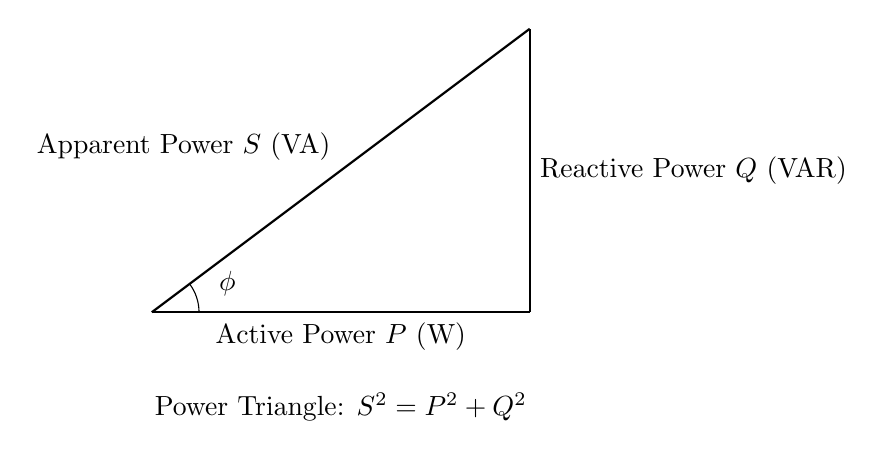
\begin{tikzpicture}[scale=1.2]
    \draw[thick] (0,0) -- (4,0) node[midway, below] {Active Power $P$ (W)};
    \draw[thick] (4,0) -- (4,3) node[midway, right] {Reactive Power $Q$ (VAR)};
    \draw[thick] (0,0) -- (4,3) node[midway, above left] {Apparent Power $S$ (VA)};
    \draw (0.5,0) arc (0:36.87:0.5);
    \node at (0.8, 0.3) {$\phi$};
    \node at (2, -1) {Power Triangle: $S^2 = P^2 + Q^2$};
\end{tikzpicture}
\end{answerdiagram}
\end{solutionbox}

\begin{mnemonicbox}
\mnemonic{PAWS: Power Active Works, Apparent is Slant-hypotenuse, reactive Qoscillates}
\end{mnemonicbox}

\questionmarks{2(c)}{7}{Explain concept of cell and battery. List out various rating and types of battery.}

\begin{solutionbox}
\textbf{Answer}:

\textbf{Difference:}
\begin{itemize}
    \item \keyword{Cell}: Basic electrochemical unit that converts chemical energy to electrical energy.
    \item \keyword{Battery}: Collection of one or more cells connected in series (for voltage) or parallel (for current).
\end{itemize}

\textbf{Battery Ratings:}
\begin{itemize}
    \item \keyword{Voltage}: Potential difference (Volts, V).
    \item \keyword{Capacity}: Amount of charge stored (Ampere-hour, Ah).
    \item \keyword{Energy}: Total energy available (Watt-hour, Wh).
    \item \keyword{C-Rate}: Rate of charge/discharge relative to capacity.
    \item \keyword{Cycle Life}: Number of charge/discharge cycles before degradation.
\end{itemize}

\begin{answerdiagram}{Battery Classification}
\begin{tikzpicture}[
    level 1/.style={sibling distance=4cm},
    level 2/.style={sibling distance=1.5cm}
]
\node [gtu root] {Battery Types}
    child { node [gtu child] {Primary\\(Non-rechargeable)}
        child { node [gtu child] {Alkaline} }
        child { node [gtu child] {Zinc-Carbon} }
        child { node [gtu child] {Lithium} }
    }
    child { node [gtu child] {Secondary\\(Rechargeable)}
        child { node [gtu child] {Lead-Acid} }
        child { node [gtu child] {Li-ion} }
        child { node [gtu child] {Ni-MH} }
    };
\end{tikzpicture}
\end{answerdiagram}
\end{solutionbox}

\begin{mnemonicbox}
\mnemonic{CAVE: Cells Are Voltage Elements, batteries Bundle And TallY Energy}
\end{mnemonicbox}

% Question 2 OR
\questionmarks{2(a) OR}{3}{Define the terms resistance, conductance and conductivity.}

\begin{solutionbox}
\textbf{Answer}:

\begin{center}
\captionof{table}{Electrical Material Properties}
\begin{tabulary}{\linewidth}{|L|L|L|L|}
\hline
\textbf{Term} & \textbf{Definition} & \textbf{Unit} & \textbf{Formula} \\ \hline
\textbf{Resistance (R)} & Opposition offered by material to flow of current. & Ohm ($\Omega$) & $R = \rho l/A$ \\ \hline
\textbf{Conductance (G)} & Reciprocal of resistance; ease of current flow. & Siemens (S) & $G = 1/R$ \\ \hline
\textbf{Conductivity ($\sigma$)} & Material property representing ability to conduct current. & S/m & $\sigma = 1/\rho$ \\ \hline
\end{tabulary}
\end{center}

Where $\rho$ is resistivity.
\end{solutionbox}

\begin{mnemonicbox}
\mnemonic{RCG: Resist Current Gladly, Conduct Generously, Sigma Gets current through}
\end{mnemonicbox}

\questionmarks{2(b) OR}{4}{Prove that for pure inductive circuit, the current lags applied voltage by 90°.}

\begin{solutionbox}
\textbf{Answer}:

Consider a pure inductive circuit with inductance $L$.

\begin{itemize}
    \item Applied Voltage: $v = V_m \sin(\omega t)$
    \item For an inductor, the back EMF opposes voltage: $v = L \frac{di}{dt}$
    \item Rearranging for current: $di = \frac{v}{L} dt = \frac{V_m}{L} \sin(\omega t) dt$
    \item Integrating both sides:
    \[ i = \int \frac{V_m}{L} \sin(\omega t) dt = -\frac{V_m}{\omega L} \cos(\omega t) \]
    \[ i = \frac{V_m}{\omega L} \sin(\omega t - 90^\circ) \]
    \item This shows current $i$ lags voltage $v$ by $90^\circ$.
\end{itemize}

\begin{answerdiagram}{Inductive Circuit Waveforms}
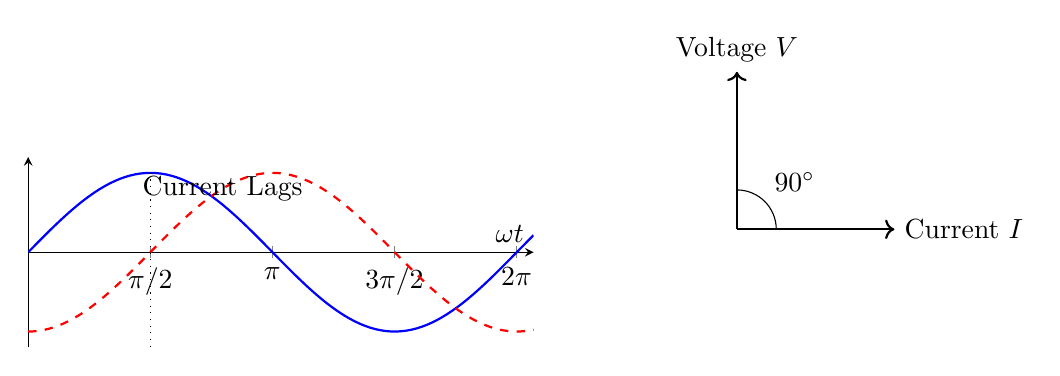
\begin{tikzpicture}
    \begin{axis}[
        width=8cm, height=4cm,
        axis lines=middle,
        xtick={0, 1.57, 3.14, 4.71, 6.28},
        xticklabels={0, $\pi/2$, $\pi$, $3\pi/2$, $2\pi$},
        ytick=\empty,
        xlabel=$\omega t$,
        ymin=-1.2, ymax=1.2
    ]
    \addplot[blue, thick, domain=0:6.5, samples=100] {sin(deg(x))} node[right] {$v$};
    \addplot[red, thick, dashed, domain=0:6.5, samples=100] {sin(deg(x)-90)} node[right] {$i$};
    \draw[dotted] (axis cs:1.57, 1) -- (axis cs:1.57, -1.2);
    \node at (axis cs:2.5, 0.8) {Current Lags};
    \end{axis}
    
    \begin{scope}[xshift=9cm, yshift=1.5cm]
        \draw[->, thick] (0,0) -- (2,0) node[right] {Current $I$};
        \draw[->, thick] (0,0) -- (0,2) node[above] {Voltage $V$};
        \draw (0.5,0) arc (0:90:0.5) node[midway, above right] {$90^\circ$};
    \end{scope}
\end{tikzpicture}
\end{answerdiagram}
\end{solutionbox}

\begin{mnemonicbox}
\mnemonic{ELI: Voltage Leads current In inductor by 90 degrees}
\end{mnemonicbox}

\questionmarks{2(c) OR}{7}{Describe Resistor, Inductor and Capacitor with their formula.}

\begin{solutionbox}
\textbf{Answer}:

\begin{center}
\captionof{table}{Passive Circuit Components}
\begin{tabulary}{\linewidth}{|L|L|L|L|L|}
\hline
\textbf{Component} & \textbf{Parameter} & \textbf{Description} & \textbf{V-I Formula} & \textbf{Energy} \\ \hline
\textbf{Resistor} & Resistance (R) & Opposes flow of current, dissipates energy as heat. & $V = IR$ & None (Dissipates) \\ \hline
\textbf{Inductor} & Inductance (L) & Opposes change in current, stores energy in magnetic field. & $V = L\frac{di}{dt}$ & $E = \frac{1}{2}LI^2$ \\ \hline
\textbf{Capacitor} & Capacitance (C) & Opposes change in voltage, stores energy in electric field. & $I = C\frac{dv}{dt}$ & $E = \frac{1}{2}CV^2$ \\ \hline
\end{tabulary}
\end{center}

\textbf{Effect on AC Circuit:}
\begin{itemize}
    \item \keyword{Resistor}: Current in phase with voltage. Power Factor = 1.
    \item \keyword{Inductor}: Current lags voltage by $90^\circ$. Power Factor = 0 lagging.
    \item \keyword{Capacitor}: Current leads voltage by $90^\circ$. Power Factor = 0 leading.
\end{itemize}

\begin{answerdiagram}{R, L, C Symbols and AC Response}
\begin{circuitikz}
    \draw (0,2) to[R, l=$R$] (2,2);
    \node at (1,1.5) {$V, I$ In Phase};
    
    \draw (3,2) to[L, l=$L$] (5,2);
    \node at (4,1.5) {$I$ Lags $V$};
    
    \draw (6,2) to[C, l=$C$] (8,2);
    \node at (7,1.5) {$I$ Leads $V$};
    
    % Vector mini-diagrams
    \draw[->] (1,0) -- (2,0) node[right] {$V, I$}; % R
    
    \draw[->] (4,0) -- (5,0) node[right] {$I$}; % L
    \draw[->] (4,0) -- (4,1) node[midway, left] {$V$};
    
    \draw[->] (7,0) -- (8,0) node[right] {$V$}; % C
    \draw[->] (7,0) -- (7,1) node[midway, left] {$I$};
\end{circuitikz}
\end{answerdiagram}
\end{solutionbox}

\begin{mnemonicbox}
\mnemonic{RIC: Resistor Impedes Current, Inductor Catches current-changes, Capacitor Controls voltage-changes}
\end{mnemonicbox}

% Question 3
\questionmarks{3(a)}{3}{Define and explain R.M.S value and average value of AC signal.}

\begin{solutionbox}
\textbf{Answer}:

\begin{center}
\captionof{table}{RMS vs Average Value}
\begin{tabulary}{\linewidth}{|L|L|L|L|}
\hline
\textbf{Value} & \textbf{Definition} & \textbf{Formula (Sine Wave)} & \textbf{Relation} \\ \hline
\textbf{RMS Value} & Square root of mean of squared values. & $V_{rms} = \frac{V_{max}}{\sqrt{2}} = 0.707 V_{max}$ & Equivalent DC heating effect. \\ \hline
\textbf{Average Value} & Mean of rectified signal over half cycle. & $V_{avg} = \frac{2V_{max}}{\pi} = 0.637 V_{max}$ & Used for battery charging. \\ \hline
\end{tabulary}
\end{center}
\end{solutionbox}

\begin{mnemonicbox}
\mnemonic{RAM: Rms-Average Method: Root-mean-square And Mean-of-absolute}
\end{mnemonicbox}

\questionmarks{3(b)}{4}{With necessary diagrams explain how alternating EMF is generated?}

\begin{solutionbox}
\textbf{Answer}:

\textbf{Principle}: When a coil rotates in a uniform magnetic field, the magnetic flux linking with it changes, inducing an EMF (Faraday's Law).

\begin{answerdiagram}{AC EMF Generation}
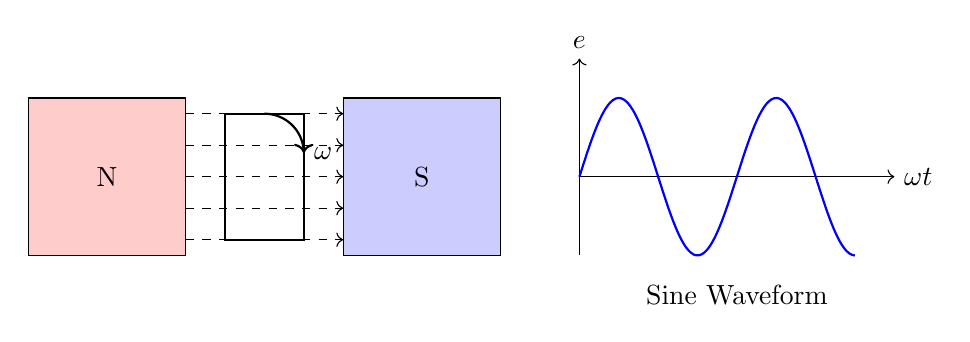
\begin{tikzpicture}
    % Magnets
    \draw[fill=red!20] (-3,-1) rectangle (-1,1) node[midway] {N};
    \draw[fill=blue!20] (1,-1) rectangle (3,1) node[midway] {S};
    
    % Field Lines
    \foreach \y in {-0.8,-0.4,0,0.4,0.8}
        \draw[dashed, ->] (-1,\y) -- (1,\y);

    % Coil
    \draw[thick] (-0.5,-0.8) rectangle (0.5,0.8);
    \draw[->, thick] (0,0.8) arc (90:0:0.5) node[right] {$\omega$};
    
    % Waveform
    \begin{scope}[xshift=4cm, yshift=-1cm]
        \draw[->] (0,1) -- (4,1) node[right] {$\omega t$};
        \draw[->] (0,0) -- (0,2.5) node[above] {$e$};
        \draw[blue, thick, smooth, samples=100, domain=0:3.5] plot (\x, {1 + sin(\x*180)});
        \node at (2, -0.5) {Sine Waveform};
    \end{scope}
\end{tikzpicture}
\end{answerdiagram}

\begin{itemize}
    \item Coil rotates, cutting flux ($\phi$).
    \item $e = -N \frac{d\phi}{dt} = N B A \omega \sin(\omega t)$.
    \item Direction changes every half cycle.
\end{itemize}
\end{solutionbox}

\begin{mnemonicbox}
\mnemonic{FARM: Flux And Rotation Make alternating voltage}
\end{mnemonicbox}

\questionmarks{3(c)}{7}{Explain A.C analysis of purely resistive AC circuit.}

\begin{solutionbox}
\textbf{Answer}:

\textbf{Purely Resistive Circuit:}
\begin{itemize}
    \item Applied Voltage: $v = V_m \sin \omega t$
    \item Current: $i = \frac{v}{R} = \frac{V_m}{R} \sin \omega t = I_m \sin \omega t$
\end{itemize}

\begin{center}
\captionof{table}{Resistive Circuit Analysis}
\begin{tabulary}{\linewidth}{|L|L|L|}
\hline
\textbf{Parameter} & \textbf{Formula} & \textbf{Relationship} \\ \hline
\textbf{Voltage} & $v = V_m \sin \omega t$ & In Phase with Current \\ \hline
\textbf{Current} & $i = I_m \sin \omega t$ & Follows Ohm's Law \\ \hline
\textbf{Power} & $p = vi = V_m I_m \sin^2 \omega t$ & Always positive \\ \hline
\textbf{Avg Power} & $P = V_{rms} I_{rms} = I^2R$ & Constant heating \\ \hline
\end{tabulary}
\end{center}

\begin{answerdiagram}{Resistive Circuit Waveforms}
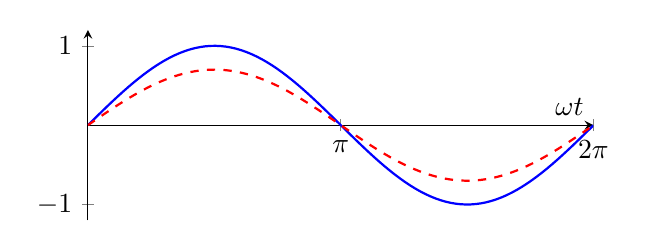
\begin{tikzpicture}
    \begin{axis}[
        width=8cm, height=4cm,
        axis lines=middle,
        xtick={0, 3.14, 6.28},
        xticklabels={0, $\pi$, $2\pi$},
        xlabel=$\omega t$,
        ymin=-1.2, ymax=1.2
    ]
    \addplot[blue, thick, domain=0:6.28, samples=100] {sin(deg(x))} node[right] {$v$};
    \addplot[red, thick, dashed, domain=0:6.28, samples=100] {0.7*sin(deg(x))} node[right] {$i$};
    \end{axis}
\end{tikzpicture}
\end{answerdiagram}
\end{solutionbox}

\begin{mnemonicbox}
\mnemonic{VIPS: Voltage In-Phase with current, Same waveform, Power always Positive}
\end{mnemonicbox}

% Question 3 OR
\questionmarks{3(a) OR}{3}{Alternating current is given by I = 28.28sin(2$\pi$50t). Find R.M.S value of current.}

\begin{solutionbox}
\textbf{Answer}:

\textbf{Given}: $I = 28.28 \sin(2\pi 50 t)$ compare with $I = I_m \sin(\omega t)$.
\begin{itemize}
    \item $I_m = 28.28$ A
\end{itemize}

\textbf{Calculation}:
\[ I_{rms} = \frac{I_m}{\sqrt{2}} = \frac{28.28}{1.414} = 20 \text{ A} \]

\textbf{Result}: RMS Current = 20 A
\end{solutionbox}

\begin{mnemonicbox}
\mnemonic{PER: Peak to Effective by Root-2}
\end{mnemonicbox}

\questionmarks{3(b) OR}{4}{Find maximum value and R.M.S value of sinusoidal voltage if Vav=60V.}

\begin{solutionbox}
\textbf{Answer}:

\textbf{Given}: $V_{av} = 60$ V.

\begin{center}
\captionof{table}{Calculations}
\begin{tabulary}{\linewidth}{|L|L|L|}
\hline
\textbf{Step} & \textbf{Formula} & \textbf{Calculation} \\ \hline
\textbf{Find Max ($V_m$)} & $V_{av} = 0.637 V_m \implies V_m = \frac{V_{av}}{0.637}$ & $V_m = \frac{60}{0.637} = 94.2$ V \\ \hline
\textbf{Find RMS ($V_{rms}$)} & $V_{rms} = 0.707 V_m$ & $V_{rms} = 0.707 \times 94.2 = 66.6$ V \\ \hline
\end{tabulary}
\end{center}

\textbf{Result}: Max Value = 94.2 V, RMS Value = 66.6 V
\end{solutionbox}

\begin{mnemonicbox}
\mnemonic{AVR: Average to peak Via multiplying by (pi/2), Rms is peak/root2}
\end{mnemonicbox}

\questionmarks{3(c) OR}{7}{Derive equation of line and phase voltage for balanced star connected load with help of phasor diagram.}

\begin{solutionbox}
\textbf{Answer}:

\begin{answerdiagram}{Star Connection and Phasor}
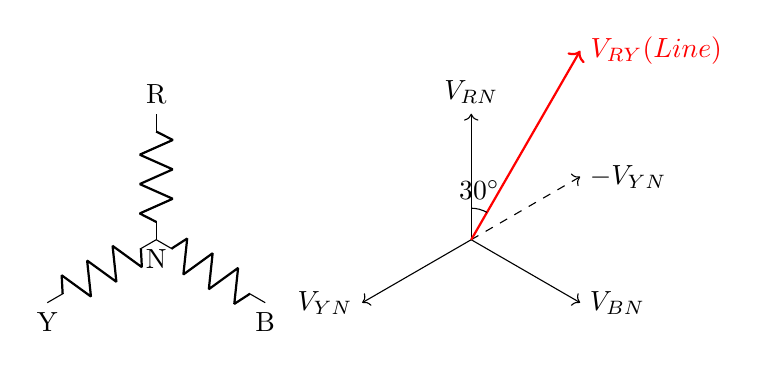
\begin{tikzpicture}[scale=0.8]
    % Star Load
    \draw (0,0) node[anchor=north]{N} to[R] (0,2) node[anchor=south]{R};
    \draw (0,0) to[R] (-1.73,-1) node[anchor=north]{Y};
    \draw (0,0) to[R] (1.73,-1) node[anchor=north]{B};
    
    % Phasor
    \begin{scope}[xshift=5cm, yshift=0cm]
        \draw[->] (0,0) -- (0,2) node[above] {$V_{RN}$};
        \draw[->] (0,0) -- (-1.73,-1) node[left] {$V_{YN}$};
        \draw[->] (0,0) -- (1.73,-1) node[right] {$V_{BN}$};
        
        \draw[dashed, ->] (0,0) -- (1.73,1) node[right] {$-V_{YN}$};
        \draw[thick, ->, red] (0,0) -- (1.73,3) node[right] {$V_{RY} (Line)$};
        \draw (0,0.5) arc (90:60:0.5) node[midway, above] {$30^\circ$};
    \end{scope}
\end{tikzpicture}
\end{answerdiagram}

\textbf{Derivation}:
\begin{itemize}
    \item Line Voltage $V_{RY}$ is vector difference of $V_{RN}$ and $V_{YN}$.
    \item $V_{RY} = V_{RN} - V_{YN}$
    \item Magnitude: $V_L = \sqrt{V_P^2 + V_P^2 + 2V_PV_P \cos(60^\circ)} = \sqrt{3V_P^2}$
    \item \keyword{Result}: $V_L = \sqrt{3} V_P$
    \item Line voltage leads Phase voltage by $30^\circ$.
\end{itemize}
\end{solutionbox}

\begin{mnemonicbox}
\mnemonic{PALS: Phase to Line in Star: multiply by Square-root-3}
\end{mnemonicbox}

% Question 4
\questionmarks{4(a)}{3}{Write statement of Faraday's law and Lenz's law with expression.}

\begin{solutionbox}
\textbf{Answer}:

\begin{center}
\captionof{table}{Laws of Induction}
\begin{tabulary}{\linewidth}{|L|L|L|}
\hline
\textbf{Law} & \textbf{Statement} & \textbf{Expression} \\ \hline
\textbf{Faraday's Law} & INDUCED EMF is directly proportional to the rate of change of magnetic flux. & $e = -N \frac{d\phi}{dt}$ \\ \hline
\textbf{Lenz's Law} & The direction of induced EMF opposes the cause producing it (indicated by negative sign). & Negative sign in $e = -N \frac{d\phi}{dt}$ \\ \hline
\end{tabulary}
\end{center}
\end{solutionbox}

\begin{mnemonicbox}
\mnemonic{FORC: Faraday's flux Over Rate Change, Lenz Opposes the Reason for Change}
\end{mnemonicbox}

\questionmarks{4(b)}{4}{State any four advantage of 3-phase supply over single-phase supply.}

\begin{solutionbox}
\textbf{Answer}:

\begin{itemize}
    \item \keyword{Higher Power Density}: For same size, 3-phase machine produces more power.
    \item \keyword{Constant Power}: 3-phase power is constant (non-pulsating), unlike 1-phase.
    \item \keyword{Material Saving}: Requires less copper for same power transmission.
    \item \keyword{Self-Starting}: 3-phase motors are self-starting due to rotating magnetic field.
\end{itemize}
\end{solutionbox}

\begin{mnemonicbox}
\mnemonic{PCCS: Power higher, Constant delivery, Copper less, Self-starting motors}
\end{mnemonicbox}

\questionmarks{4(c)}{7}{Explain Fleming's right-hand rule for generators and left-hand rule for motors.}

\begin{solutionbox}
\textbf{Answer}:

\begin{center}
\captionof{table}{Fleming's Rules Comparison}
\begin{tabulary}{\linewidth}{|L|L|L|}
\hline
\textbf{Feature} & \textbf{Right-Hand Rule (Generator)} & \textbf{Left-Hand Rule (Motor)} \\ \hline
\textbf{Purpose} & Find Induced EMF/Current Direction & Find Force/Motion Direction \\ \hline
\textbf{Thumb} & Motion of Conductor & Motion/Force \\ \hline
\textbf{Forefinger} & Magnetic Field (N to S) & Magnetic Field (N to S) \\ \hline
\textbf{Middle Finger} & Induced Current & Current \\ \hline
\end{tabulary}
\end{center}

\begin{answerdiagram}{Fleming's Hand Rules}
\begin{tikzpicture}
    % Right Hand
    \begin{scope}[xshift=0cm]
        \draw[->, Ultra Thick, blue] (0,0) -- (0,2) node[above] {Motion};
        \draw[->, Ultra Thick, red] (0,0) -- (2,0) node[right] {Field};
        \draw[->, Ultra Thick, purple] (0,0) -- (0,0,-2) node[left] {Induced Current};
        \node at (0,-1) {Right Hand (Generator)};
    \end{scope}

    % Left Hand
    \begin{scope}[xshift=5cm]
        \draw[->, Ultra Thick, blue] (0,0) -- (0,2) node[above] {Force/Motion};
        \draw[->, Ultra Thick, red] (0,0) -- (2,0) node[right] {Field};
        \draw[->, Ultra Thick, green!60!black] (0,0) -- (0,0,-2) node[left] {Current};
        \node at (0,-1) {Left Hand (Motor)};
    \end{scope}
\end{tikzpicture}
\end{answerdiagram}
\end{solutionbox}

\begin{mnemonicbox}
\mnemonic{FBI-MFC: Field-B-Induced current for right hand, Motion-Field-Current for left}
\end{mnemonicbox}

% Question 4 OR
\questionmarks{4(a) OR}{3}{Describe phenomenon of electromagnetic induction.}

\begin{solutionbox}
\textbf{Answer}:

\keyword{Electromagnetic Induction}: The process of generating an electromotive force (EMF) across a conductor when it is exposed to a changing magnetic field.

\begin{answerdiagram}{Induction Flow}
\begin{tikzpicture}[node distance=1.5cm, auto]
    \node [gtu block] (flux) {Changing Flux};
    \node [gtu block, right=of flux] (emf) {Induced EMF};
    \node [gtu block, right=of emf] (current) {Induced Current};
    
    \path [gtu arrow] (flux) -- (emf);
    \path [gtu arrow] (emf) -- (current);
\end{tikzpicture}
\end{answerdiagram}
\end{solutionbox}

\begin{mnemonicbox}
\mnemonic{MICE: Motion Induces Current via Electromagnetic induction}
\end{mnemonicbox}

\questionmarks{4(b) OR}{4}{Explain the generation of 3-phase alternating EMF.}

\begin{solutionbox}
\textbf{Answer}:

\textbf{Generation Principle}:
\begin{itemize}
    \item Three coils placed at $120^\circ$ electrical displacement in space.
    \item Rotating these coils in a magnetic field induces three EMFs.
    \item EMFs have same magnitude and frequency but are phase-shifted by $120^\circ$.
\end{itemize}

\begin{answerdiagram}{3-Phase Waveforms}
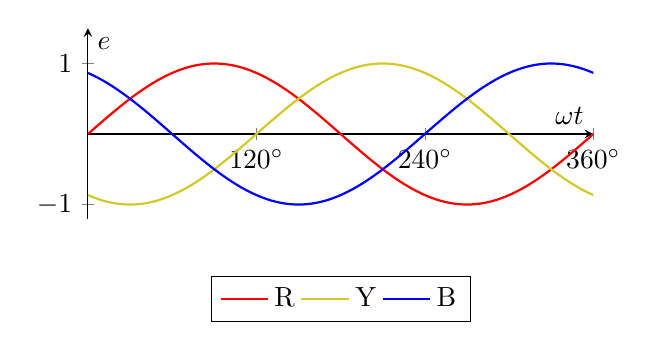
\begin{tikzpicture}
    \begin{axis}[
        width=8cm, height=4cm,
        axis lines=middle,
        xtick={0, 120, 240, 360},
        xticklabels={0, $120^\circ$, $240^\circ$, $360^\circ$},
        xlabel=$\omega t$,
        ylabel=$e$,
        ymin=-1.2, ymax=1.5,
        legend style={at={(0.5,-0.3)}, anchor=north, legend columns=-1}
    ]
    \addplot[red, thick, domain=0:360, samples=100] {sin(x)}; \addlegendentry{R}
    \addplot[yellow!80!black, thick, domain=0:360, samples=100] {sin(x-120)}; \addlegendentry{Y}
    \addplot[blue, thick, domain=0:360, samples=100] {sin(x-240)}; \addlegendentry{B}
    \end{axis}
\end{tikzpicture}
\end{answerdiagram}
\end{solutionbox}

\begin{mnemonicbox}
\mnemonic{CPS: Coils Produce Shifted waveforms at 120 degrees}
\end{mnemonicbox}

\questionmarks{4(c) OR}{7}{Differentiate statically and dynamically induced E.M.F.}

\begin{solutionbox}
\textbf{Answer}:

\begin{center}
\captionof{table}{Static vs Dynamic EMF}
\begin{tabulary}{\linewidth}{|L|L|L|}
\hline
\textbf{Parameter} & \textbf{Statically Induced EMF} & \textbf{Dynamically Induced EMF} \\ \hline
\textbf{Definition} & EMF induced without moving parts (change in flux linkage). & EMF induced by relative motion between conductor and field. \\ \hline
\textbf{Motion} & Stationary conductor and field. & Moving conductor or field. \\ \hline
\textbf{Formula} & $e = -N \frac{d\phi}{dt}$ & $e = Blv \sin \theta$ \\ \hline
\textbf{Example} & Transformer & Generator, DC Dynamo \\ \hline
\end{tabulary}
\end{center}
\end{solutionbox}

\begin{mnemonicbox}
\mnemonic{SMCE: Static-Moving, Change-External: static has changing flux, moving has constant flux}
\end{mnemonicbox}

% Question 5
\questionmarks{5(a)}{3}{Differentiate HAWT and VAWT.}

\begin{solutionbox}
\textbf{Answer}:

\begin{center}
\captionof{table}{HAWT vs VAWT}
\begin{tabulary}{\linewidth}{|L|L|L|}
\hline
\textbf{Parameter} & \textbf{HAWT (Horizontal Axis)} & \textbf{VAWT (Vertical Axis)} \\ \hline
\textbf{Axis} & Horizontal (parallel to ground) & Vertical (perpendicular to ground) \\ \hline
\textbf{Wind Direction} & Needs Yaw mechanism to face wind. & Omni-directional (accepts wind from any side). \\ \hline
\textbf{Generation} & Components at top of tower. & Generator can be on ground. \\ \hline
\end{tabulary}
\end{center}

\begin{answerdiagram}{Wind Turbine Types}
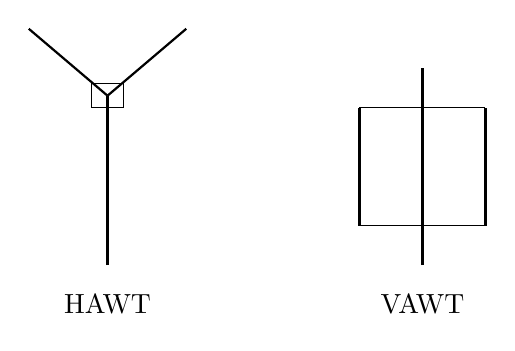
\begin{tikzpicture}
    % HAWT
    \begin{scope}[xshift=0cm]
        \draw[thick] (0,0) -- (0,2); % Tower
        \draw[fill=white] (-0.2,2) rectangle (0.2,2.3); % Nacelle
        \draw[thick] (0,2.15) -- (-1,3); % Blade 1
        \draw[thick] (0,2.15) -- (1,3); % Blade 2
        \draw[thick] (0,2.15) -- (0,1); % Blade 3
        \node at (0,-0.5) {HAWT};
    \end{scope}

    % VAWT
    \begin{scope}[xshift=4cm]
        \draw[thick] (0,0) -- (0,2.5); % Shaft
        \draw[thick] (-0.8,0.5) to[out=90,in=270] (-0.8,2); % Blade L
        \draw[thick] (0.8,0.5) to[out=90,in=270] (0.8,2); % Blade R
        \draw (-0.8,0.5) -- (0.8,0.5);
        \draw (-0.8,2) -- (0.8,2);
        \node at (0,-0.5) {VAWT};
    \end{scope}
\end{tikzpicture}
\end{answerdiagram}
\end{solutionbox}

\begin{mnemonicbox}
\mnemonic{HV-DIT: Horizontal-Vertical, Directional-Independent, Tall-lower}
\end{mnemonicbox}

\questionmarks{5(b)}{4}{Classification of green energy.}

\begin{solutionbox}
\textbf{Answer}:

\begin{itemize}
    \item \keyword{Solar Energy}: Photovoltaic, Thermal.
    \item \keyword{Wind Energy}: Onshore, Offshore.
    \item \keyword{Hydro Energy}: Dams, Tidal, Wave.
    \item \keyword{Geothermal}: Earth's heat.
    \item \keyword{Biomass}: Organic waste.
\end{itemize}

\begin{answerdiagram}{Green Energy Classification}
\begin{tikzpicture}[
    level 1/.style={sibling distance=2.2cm, level distance=1.5cm},
    edge from parent fork down
]
\node [gtu root] {Green Energy}
    child { node [gtu child] {Solar} }
    child { node [gtu child] {Wind} }
    child { node [gtu child] {Hydro} }
    child { node [gtu child] {Bio} }
    child { node [gtu child] {Geo} };
\end{tikzpicture}
\end{answerdiagram}
\end{solutionbox}

\begin{mnemonicbox}
\mnemonic{SWHGBT: Sun Wind Hydro Geo Bio Tidal - Sources With Huge Green Benefits Today}
\end{mnemonicbox}

\questionmarks{5(c)}{7}{Explain wind power system.}

\begin{solutionbox}
\textbf{Answer}:

\textbf{Components}:
\begin{enumerate}
    \item \keyword{Blades}: Capture wind energy (Aerodynamic).
    \item \keyword{Rotor}: Hub connecting blades.
    \item \keyword{Gearbox}: Increases speed for generator.
    \item \keyword{Generator}: Converts mechanical rotation to electricity.
    \item \keyword{Yaw Drive}: Orients turbine towards wind.
    \item \keyword{Tower}: Supports assembly at height.
\end{enumerate}

\begin{answerdiagram}{Wind Power Block Diagram}
\begin{tikzpicture}[node distance=1.2cm, auto]
    \node [gtu block] (wind) {Wind};
    \node [gtu block, right=of wind] (blade) {Blades/Rotor};
    \node [gtu block, right=of blade] (gear) {Gearbox};
    \node [gtu block, right=of gear] (gen) {Generator};
    \node [gtu block, below=of gen] (grid) {Grid};
    
    \path [gtu arrow] (wind) -- (blade);
    \path [gtu arrow] (blade) -- (gear);
    \path [gtu arrow] (gear) -- (gen);
    \path [gtu arrow] (gen) -- (grid);
    
    \node [draw, dashed, fit=(blade) (gear) (gen)] (nacelle) {};
    \node [above] at (nacelle.north) {Nacelle};
\end{tikzpicture}
\end{answerdiagram}
\end{solutionbox}

\begin{mnemonicbox}
\mnemonic{WINGER: Wind In, Gearbox Enhances Rotation, Generator outputs}
\end{mnemonicbox}

% Question 5 OR
\questionmarks{5(a) OR}{3}{List any three needs of green energy.}

\begin{solutionbox}
\textbf{Answer}:

\begin{itemize}
    \item \keyword{Environmental Protection}: Reduce carbon footprint and pollution.
    \item \keyword{Sustainability}: Infinite source compared to fossil fuels.
    \item \keyword{Energy Security}: Reduce dependence on imported fuels.
\end{itemize}
\end{solutionbox}

\begin{mnemonicbox}
\mnemonic{ECO: Environment protected, Conservation of resources, Oil-independence}
\end{mnemonicbox}

\questionmarks{5(b) OR}{4}{Write short note on PV cell.}

\begin{solutionbox}
\textbf{Answer}:

\textbf{Photovoltaic (PV) Cell}:
\begin{itemize}
    \item Basic unit of solar system.
    \item Made of Semiconductor (Silicon).
    \item Works on \keyword{Photovoltaic Effect}: Photons strike PN junction $\to$ electron-hole pairs $\to$ Current.
    \item Output: DC voltage (~0.5-0.6V per cell).
\end{itemize}

\begin{answerdiagram}{PV Cell Construction}
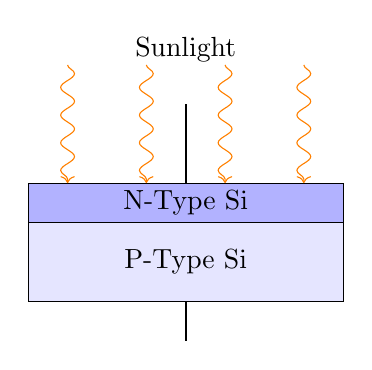
\begin{tikzpicture}
    \draw[fill=blue!10] (0,0) rectangle (4,1) node[midway] {P-Type Si};
    \draw[fill=blue!30] (0,1) rectangle (4,1.5) node[midway] {N-Type Si};
    \draw[thick] (2,1.5) -- (2,2.5); % Wire
    \draw[thick] (2,-0.5) -- (2,0);
    \foreach \x in {0.5, 1.5, 2.5, 3.5}
        \draw[->, orange, decorate, decoration={snake}] (\x,3) -- (\x,1.5);
    \node at (2, 3.2) {Sunlight};
\end{tikzpicture}
\end{answerdiagram}
\end{solutionbox}

\begin{mnemonicbox}
\mnemonic{SPEC: Sunlight Produces Electricity through Cells with p-n junctions}
\end{mnemonicbox}

\questionmarks{5(c) OR}{7}{Explain solar system.}

\begin{solutionbox}
\textbf{Answer}:

\textbf{Solar Power System}:
\begin{enumerate}
    \item \keyword{Solar Array}: Collection of PV panels to generate DC.
    \item \keyword{Charge Controller}: Regulates voltage/current to battery.
    \item \keyword{Battery Bank}: Stores energy for later use (Off-grid).
    \item \keyword{Inverter}: Converts DC to AC for appliances.
    \item \keyword{Load}: Electrical devices.
\end{enumerate}

\begin{answerdiagram}{Solar System Block Diagram}
\begin{tikzpicture}[node distance=1.5cm, auto]
    \node [gtu block] (panel) {PV Panels};
    \node [gtu block, right=of panel] (cc) {Charge Controller};
    \node [gtu block, below=of cc] (batt) {Battery};
    \node [gtu block, right=of cc] (inv) {Inverter};
    \node [gtu block, right=of inv] (load) {AC Load};
    
    \path [gtu arrow] (panel) -- (cc);
    \path [gtu arrow] (cc) -- (batt);
    \path [gtu arrow] (cc) -- (inv);
    \path [gtu arrow] (inv) -- (load);
    \path [gtu arrow] (batt) -- (cc);
\end{tikzpicture}
\end{answerdiagram}
\end{solutionbox}

\begin{mnemonicbox}
\mnemonic{SCBID: Solar Cells produce, Battery stores, Inverter converts, Distribution supplies}
\end{mnemonicbox}

\end{document}


